%%%%%%%%%%%%%%%%%%%%%%%%%%%%%%%%
% Operazioni sulle Descrizioni %
%%%%%%%%%%%%%%%%%%%%%%%%%%%%%%%%
\section{Operazioni sulle Descrizioni}

%%%%%%%%%%%%%%%%%%%%%%%%%%%%%%
%   Visualizza Descrizione   %
%%%%%%%%%%%%%%%%%%%%%%%%%%%%%%
\subsection{Visualizzazione}
\begin{itemize}
	\item \textbf{Operazione}: visualizzaDescrizione
	\item \textbf{Obiettivo}: Visualizza la Descrizione di un'Opera, dato il suo IdDescr
	\item \textbf{Parametri}:
	\begin{enumerate}
		\item \textbf{DescrID}: in number(5)
	\end{enumerate}
	\item \textbf{Risultato}: Visualizza i dettagli della Descrizione richiesta, altrimenti restituisce errore
	\item \textbf{Errori}: 
	\begin{itemize}
		\item La descrizione richiesta non è presente nella base di dati
	\end{itemize}
	\item \textbf{Usa}: Descrizioni
	\item \textbf{Modifica}: Descrizioni
	\item \textbf{Precondizioni}:
	\begin{itemize}
		\item $\exists x \in Descrizioni : x.IdDescr = DescrID$
	\end{itemize}
	\item \textbf{Postcondizioni}: nessuna
\end{itemize}

%%%%%%%%%%%%%%%%%%%%%%%%%%%%%%
%   Inserisci Descrizione   %
%%%%%%%%%%%%%%%%%%%%%%%%%%%%%%
\subsection{Inserimento}
\begin{itemize}
	\item \textbf{Operazione}: inserisciDescrizione
	\item \textbf{Obiettivo}: Inserisce una nuova descrizione, associandola ad un'Opera
	\item \textbf{Parametri}:
	\begin{enumerate}
		\item \textbf{lingua}: in varchar2(25)
		\item \textbf{livello}: in varchar2(25)
		\item \textbf{testodescr}: in CLOB
		\item \textbf{OperaID}: in number(5)
	\end{enumerate}
	\item \textbf{Risultato}: Inserisce la descrizione dell'Opera, restituisce errore se l'Opera non è presente nel database
	\item \textbf{Errori}: 
	\begin{itemize}
		\item L'Opera a cui associare la descrizione non è presente nella base di dati
	\end{itemize}
	\item \textbf{Usa}: Descrizioni, Opere
	\item \textbf{Modifica}: Descrizioni
	\item \textbf{Precondizioni}:
	\begin{itemize}
		\item $\exists x \in Opere : x.IdOpera = OperaID$
	\end{itemize}
	\item \textbf{Postcondizioni}:
	\begin{itemize}
		\item $\exists x \in Descrizioni : x.Opera = OperaID \land x.Lingua = lingua \land x.Livello = livello \land x.Testo = testodescr$
	\end{itemize}
\end{itemize}
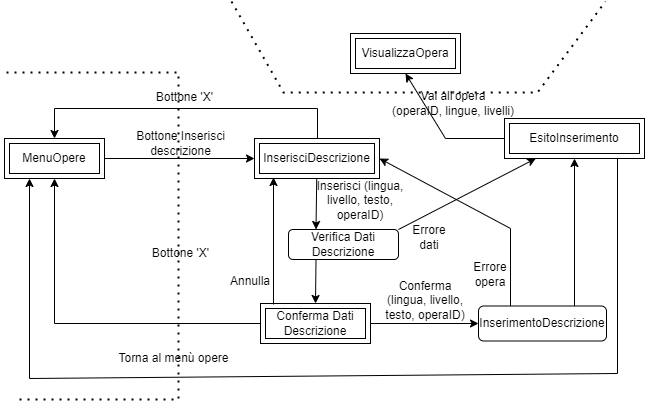
\includegraphics[width=\textwidth]{img/InserDescr.png}\\[1cm]


%%%%%%%%%%%%%%%%%%%%%%%%%%%%%%
%    Modifica Descrizione    %
%%%%%%%%%%%%%%%%%%%%%%%%%%%%%%
\subsection{Modifica}
\begin{itemize}
	\item \textbf{Operazione}: ModificaDescrizione
	\item \textbf{Obiettivo}: Modifica la descrizione di un'opera (è possibile modificare anche l'opera a cui una descrizione è associata)
	\item \textbf{Parametri}:
	\begin{enumerate}
		\item \textbf{descrID}: in number(5)
		\item \textbf{newlang}: in varchar2(25) default null
		\item \textbf{newlevel}: in varchar2(25) default null
		\item \textbf{newtext}: in CLOB default null
		\item \textbf{newOpera}: in number(5) default null
	\end{enumerate}
	\item \textbf{Risultato}: Modifica gli attributi della descrizione individuata da descrID, oppure ritorna un errore
	\item \textbf{Errori}: 
	\begin{itemize}
		\item La descrizione da modificare non è presente nella base di dati
		\item La nuova Opera da associare alla descrizione non è presente nella base di dati
	\end{itemize}
	\item \textbf{Usa}: Opere, Descrizioni
	\item \textbf{Modifica}: Descrizioni
	\item \textbf{Precondizioni}:
	\begin{itemize}
		\item $\exists x \in Descrizioni : x.IdDescr = descrID$
		\item $\exists x \in Opere : x.IdOpera = newOpera$
	\end{itemize}
	\item \textbf{Postcondizioni}:
	\begin{align*} (\exists x \in Descrizioni.
		& (newlang \ne null \Rightarrow x.Lingua = newlang) \\
		& \land (newlevel \ne null \Rightarrow x.Livello = newlevel) \\
		& \land (newtext \ne null \Rightarrow x.Testo = newtext) \\
		& \land (newOpera \ne null \Rightarrow x.Opera = newOpera))
	\end{align*}
\end{itemize}
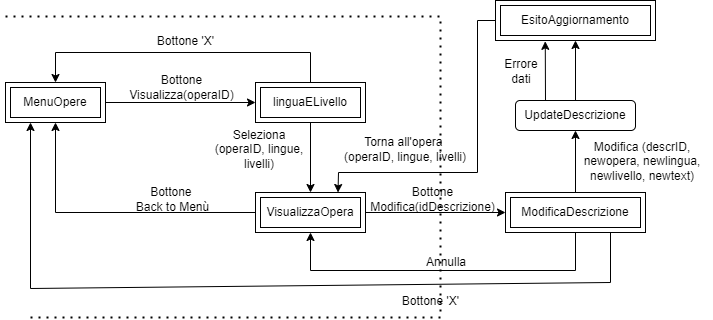
\includegraphics[width=\textwidth]{img/UpdateDescr.png}\\[1cm]


%%%%%%%%%%%%%%%%%%%%%%%%%%%%%%
%   Rimozione Descrizione    %
%%%%%%%%%%%%%%%%%%%%%%%%%%%%%%
\subsection{Rimozione}
\begin{itemize}
	\item \textbf{Operazione}: rimuoviDesrizione
	\item \textbf{Obiettivo}: Rimuove una descrizione, se presente
	\item \textbf{Parametri}:
	\begin{enumerate}
		\item \textbf{descrID}: in number(5)
	\end{enumerate}
	\item \textbf{Risultato}: Rimuove la descrizione dell'Opera, restituendo errore se la descrizione non è presente nel database
	\item \textbf{Errori}: 
	\begin{itemize}
		\item La Descrizione identificata da descrID non è presente nella base di dati
	\end{itemize}
	\item \textbf{Usa}: Descrizioni
	\item \textbf{Modifica}: Descrizioni
	\item \textbf{Precondizioni}:
	\begin{itemize}
		\item $\exists x \in Descrizioni : x.IdDescr = descrID$
		\item $|Descrizioni| = n$
	\end{itemize}
	\item \textbf{Postcondizioni}:
	\begin{itemize}
		\item $\nexists x \in Descrizioni : x.IdDescr = descrID$
		\item $|Descrizioni| = n - 1$
	\end{itemize}
\end{itemize}
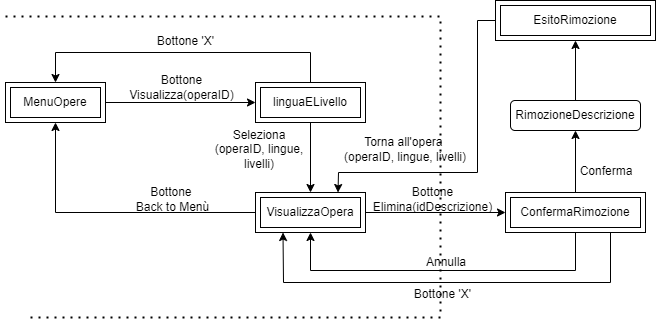
\includegraphics[width=\textwidth]{img/RimozDescr.png}\\[1cm]

%%%%%%%%%%%%%%%%%%%%%%%%%%%%%%
%   Statistiche e monitoraggio Descrizioni    %
%%%%%%%%%%%%%%%%%%%%%%%%%%%%%%
\subsection{Statistiche e monitoraggio}
\begin{itemize}
	\item \textbf{Operazione}: StatisticheDescrizioni
	\item \textbf{Obiettivo}: Visualizza le statistiche delle descrizioni
	\item \textbf{Parametri}: nessuno
	\item \textbf{Risultato}: Visualizza i titoli e le statistiche disponibili riguardanti le descrizioni
	\item \textbf{Errori}: nessuno
	\item \textbf{Usa}: Descrizioni
	\item \textbf{Modifica}: nessuna
	\item \textbf{Precondizioni}: nessuna
	\item \textbf{Postcondizioni}: nessuna
	\item \textbf{Note}: Vengono sempre eseguite tutte le operazioni di statistica
\end{itemize}

%%%%%%%%%%%%%%%%%%%%%%%%%%%%%%
%   Livello descrizione più presente    %
%%%%%%%%%%%%%%%%%%%%%%%%%%%%%%
\subsubsection{Livello descrizione più presente}
\begin{itemize}
	\item \textbf{Obiettivo}: Visualizza il livello più presente nelle descrizioni e il numero di descrizioni che lo possiedono
	\item \textbf{Parametri}: nessuno
	\item \textbf{Risultato}: Visualizza il livello di descrizione più presente e il numero di opere che lo possiedono (in caso di più livelli con il massimo valore, vengono tutti mostrati) oppure non mostra niente
	\item \textbf{Errori}: nessuno
	\item \textbf{Usa}: Descrizioni
	\item \textbf{Modifica}: nessuna
	\item \textbf{Precondizioni}: nessuna
	\item \textbf{Postcondizioni}: nessuna
\end{itemize}

%%%%%%%%%%%%%%%%%%%%%%%%%%%%%%
%   Lingua descrizione più presente    %
%%%%%%%%%%%%%%%%%%%%%%%%%%%%%%
\subsubsection{Lingua più presente}
\begin{itemize}
	\item \textbf{Obiettivo}: Visualizza la lingua più presente nelle descrizioni e il numero di descrizioni che la possiedono
	\item \textbf{Parametri}: nessuno
	\item \textbf{Risultato}: Visualizza la lingu di descrizione più presente e il numero di opere che la possiedono (in caso di più lingue con il massimo valore, vengono tutti mostrate) oppure non mostra niente
	\item \textbf{Errori}: nessuno
	\item \textbf{Usa}: Descrizioni
	\item \textbf{Modifica}: nessuna
	\item \textbf{Precondizioni}: nessuna
	\item \textbf{Postcondizioni}: nessuna
\end{itemize}
